\documentclass[a4paper]{article} 
    \title{}
    \date{} %不显示日期
    
\usepackage{xeCJK} %中文包

\usepackage{graphicx} %插入图片的宏包

\usepackage{booktabs}%加载画表格的宏包

\usepackage{floatrow} %设置表格
\floatsetup[table]{capposition=top}
\newfloatcommand{capbtabbox}{table}[][\FBwidth]

\setCJKfamilyfont{song}{SimSun} %设置字体为宋体
\usepackage{indentfirst} %首行缩进的宏包


\usepackage{geometry}   %设置页边距的宏包
\usepackage{graphics}
\geometry{left=2.5cm,right=2.5cm,top=2.5cm,bottom=2.5cm}  %设置 上、左、下、右 页边距


\usepackage{fancyhdr} %设置页眉
\pagestyle{fancy}
\lhead{ }
\chead{\bfseries 参赛队号 \#1403}
\rhead{ }
\lfoot{ }
\cfoot{\thepage}
\rfoot{ }

\renewcommand\contentsname{\centerline{目录}} %contents改为目录
\renewcommand{\baselinestretch}{1.0} %设置单倍行距

\begin{document}
	
\tableofcontents %自动生成目录
\newpage

	\section{问题重述} 
		\subsection{问题背景} 
			\paragraph{}近年来,国际保险行业稳步开展,机动车辆保险在我国的财险保费中所占比重最大,以千亿元计。并且,由于我国汽车保有辆的继续增加和相关车险的政策出台,投保率也呈继续上升趋向。车险一般可占财险公司业务的70\%到80\%,所以车险市场历来是财险公司的兵家必争之地。以往,财险公司为了赢得市场,往往采取低价、折扣来争抢客户。但是激烈的市场竞争也带来了利润率的下降,甚至有些企业在亏本经营。大多数车企为了提高利润率开始重视承保车辆的质量。重投保车辆质量的做法,其实是险企科学发展的重要体现,是市场竞争下的企业合理行为。中国目前的车险费率制度,大多数符合“从车主义”。即车险保费多少,主要取决于这辆车本身的各项情况,如车的购置价、座位数、排量、购车年限等,根据这些数据计算出一个基本的车险保费价格,再根据这辆车的上年理赔次数来打不同的折扣。这就导致了中国的车险定价模式非常的单调,相似情况的车型,保费也都差不多。
			
			\paragraph{}可以预见未来车险行业的几大发展趋势:
			\paragraph{}1.车险价格与驾驶行为密切相关 \\
			\indent 未来的车险定价将逐渐转变为“从人主义”。车险的定价因素将直接与驾
			驶人的驾驶习惯与行驶里程挂钩,通过驾驶行为来判定车险价格,可能会使
			车险由原来的一年买一次变成可以一个月买一次。一个具有良好驾驶习惯的
			车主,可能只需要支付原本保费的 30\% 左右,而驾驶习惯不佳的车主,则会
			在原本保费的基础上继续上涨。	
			\paragraph{}2. 同价位车型车险价格完全不同 \\
			\indent 国内传统的汽车保险定价,通常是以车型和其购置价为主要依据。未来中
			国车险业,同样的一款车,不同的人开,保费价格会完全不同。这个不同可能
			是取决于投保人本身的驾驶行为,还可能会以投保人本身的年龄、职业、家庭
			状况等信息为标准。信息时代的到来,为车险企业提供了一个更加有力的武器,可以通过数字
			化技术来更加精准地了解客户,制定营销和服务方案。
				
		\subsection{问题提出} 
			\paragraph{}1. 请建立合理的数学模型,对附件一中提供的客户进行精准画像,给出客户的续保概率。
			\paragraph{}2. 请针对不同的客户设计不同的优惠和福利方案,以提高续保概率。
				
	\section{符号定义} 
		$$\begin{tabular}{cc}
			\toprule  %添加表格头部粗线
			符号& 含义\\
			\midrule  %添加表格中横线
			x_1& 三者保险额\\
			x_2& 签单保费\\
			x_3& 渠道 \\
			x_4& 是否投保车损\\
			x_5& 是否投保盗抢 \\
			x_6& 是否投保车上人员\\
			x_7& 投保类别 \\
			x_8& 是否本省车牌\\
			x_9& 使用性质\\
			x_{10}& 车辆种类\\
			x_{11}& 车辆用途\\
			x_{12}& 险种\\
			x_{13}& 风险类别\\
			x_{14}& 客户类别\\
			x_{15}& 被保险人性别\\
			x_{16}& NCD \\
			x_{17}& 车龄\\
			x_{18}& 被保险人年龄 \\
			x_{19}& 立案件数 \\
			x_{20}& 已决赔款 \\
			predict()& 预测模型\\
			X& 训练样本 
			\bottomrule %添加表格底部粗线
		\end{tabular} $$
	
	\section{原理概述}
		\subsection{线性回归}
			\paragraph{}在统计学中,线性回归(Linear Regression)是利用称为线性回归方程的最小平方函数对一个或多个自变量和因变量之间关系进行建模的一种回归分析。这种函数是一个或多个称为回归系数的模型参数的线性组合。只有一个自变量的情况称为简单回归,多个自变量情况的叫做多元回归。我们的建模过程用到的是多元线性回归模型,以下是多元线性回归的公式的假设函数:\\
				$$ h_{\theta} (x) = \theta_0 x_0+\theta_1 x_1+...+\theta_n x_n \eqno{(1)}  $$  \\
			简化形式: \\
				$$ h_\theta(x)=\theta^TX \eqno{(2)} $$  \\
			其中X,$\theta$ 都是一个n阶向量。 \\
		\subsection{逻辑回归}
			\paragraph{}逻辑回归是一种广义线性模型,是一种用于解决二分类问题的机器学习方法。逻辑回归以线性回归作为理论支持,在线性回归的基础上通过sigmoid函数引入非线性元素,因此可以轻松解决0/1分类问题。引入Sigmoid函数,也称为逻辑函数:\\
				$$ g(z) = \frac{1}{1+e^{-z}} \eqno{(3)} $$   \\
			逻辑回归的假设函数形式如下:\\
			$$ h_\theta(x) = g(\theta^Tx)  \eqno{(4)} $$  
			$$ g(z) = \frac{1}{1+e^{-z}} $$ \\
			由公式(2)(4)得到 :\\
			$$ h_\theta(x) = \frac{1}{1+e^{-\theta^T}x} \eqno{(5)} $$ \\
			其中 x 是我们的输入, $\theta$ 为我们要求取的参数, x和$\theta$都是n维向量。
		\subsection{决策树}
			\paragraph{}决策树是机器学习中的一个预测模型,代表了对象属性与对象值之间的一种映射关系。决策树是一种树形结构,其中每个内部节点表示一个属性上的测试,每个分支代表一个测试输出,每个叶节点代表一种类别。决策树学习基本算法如下:
			\begin{figure}[H]	
				\centering
				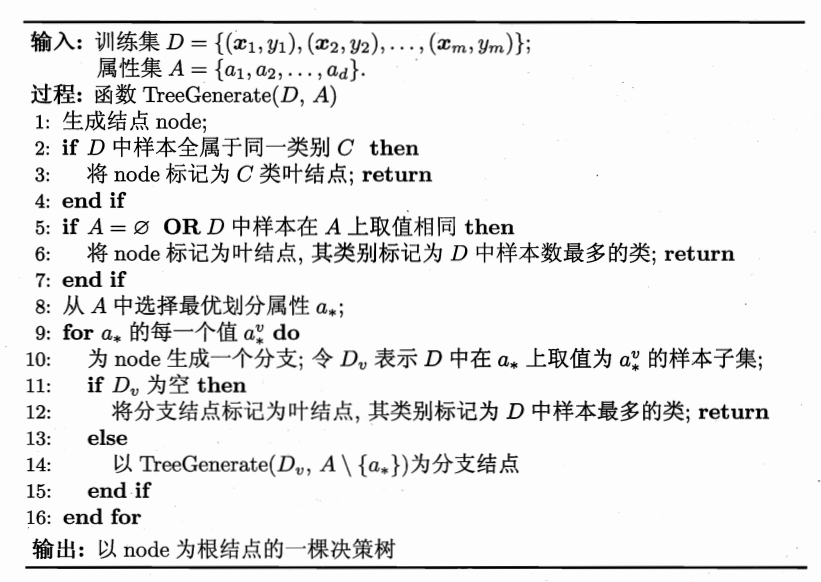
\includegraphics[scale=0.5]{tree.png}
				\caption{决策树基本学习算法}
				\label{fig:label}
			\end{figure}
			\paragraph{}显然,决策树的生成是一个递归过程。在决策树基本算法中,有三种情况会导致递归返回:(1)当前节点包含的样本全属于同一类别,无需划分;(2)当前属性集为空,或是所有样本在所有属性上取值相同无法划分;(3)当前节点包含的样本集合为空,不能划分。由Figure 1的算法可以看出,决策树学习的关键是如何选择最优划分属性。一般而言,随着划分过程不断进行,我们希望决策树的分支节点所包含的样本尽可能属于同一类别,即结点的”纯度“越来越高。“信息熵”是度量样本集合纯度最常用的一种指标。假定当前样本集合D中第k类样本所占的比例为$p_k$,(k = 1,2,...$\arrowvert$y$\arrowvert$),则D的信息熵定义为:\\
				$$ Ent(D) = -\sum_{k=1}^{\arrowvert y \arrowvert}p_klog_2P_k \eqno{(6)}$$
			Ent(D)的值越小,则D的纯度越高。
		\subsection{拉格朗日乘子法}
			\paragraph{}拉格朗日乘子法(Lagrange multipliers)是一种寻找多元函数在一组约束下的极值的方法。通过引入拉格朗日乘子,可以将d个变量与k个约束条件的最优化问题转化为具有d+k个变量的无约束优化问题求解。
			\paragraph{}引入拉格朗日乘子 $\vec \lambda=(\lambda_1,...,\lambda_m)^T$和$\mu=(\mu_1,...,\mu_n)^T$,相应的拉格朗日函数为:
				$$ L(\vec x, \vec \lambda,\vec \mu)=f(\vec x)+\sum_{i=1}^m\lambda_ih_i(\vec x)+\sum_{j=1}^n\mu_jg_j(\vec x) $$
			\indent 有不等式约束条件引入的KKT条件(j=1,2,...,n)为:
			$$ \begin{equation*}
			\left\{
			\begin{array}{lr}
			g_j(\vec x)  =  0; &  \\
			\mu_j  =  0; \\
			\mu_jg_j(\vec x)  =  0 &  
			\end{array}
			\right \eqno(7)
			\end{equation*} $$
			\paragraph{}拉格朗日”对偶函数“(dual function)$\Gamma:R\times R\mapsto R$定义为:\\
			$$ \begin{equation*}
			\begin{aligned}
			\Gamma(\vec \lambda, \vec \mu) &= inf_{x\in D}L(\vec x, \vec \lambda,\vec \mu)  \\
			&=inf_{x\in D}(f(\vec x)+\sum_{i=1}^m\lambda_ih_i(\vec x)+\sum_{j=1}^n\mu_jg_j(\vec x))
			\end{aligned} \eqno(8)
			\end{equation*}	$$
		\subsection{GradientBoostingClassifier}
			\paragraph{}梯度上升决策树模型是boost提升算法和决策树模型的结合,Gradient Boosting 采用和AdaBoost同样的加法模型,在第m次迭代中,前m-1个基学习器都是固定的,即 :
				$$ f_m(x) = f_{m-1}x + \rho_mh_m(x)$$
			因而在第m步我们的目标是最小化损失函数 $ L(f) = \sum_{i = 1}^{N}(y_i,f_m(x_i))$,进而求得相应的基学习器。若将 f(x) 当成参数,则同样可以使用梯度下降法:
				$$ f_m(x) = f_{m-1}x - \rho_m\cdot \frac{\partial}{\partial f_{m-1}x} L(y,f_{m-1}(x))$$
			对比上面两个式子,可以发现若将$h_m(x) \simeq -\frac{\partial L(y,f_{m-1}(x))}{\partial f_{m-1}(x)}$, 即即用基学习器$h_m(x)$拟合前一轮模型损失函数的负梯度,就是通过梯度下降法最小化 $L(f)$ 。由于 $f(x)$ 实际为函数,所以该方法被认为是函数空间的梯度下降。负梯度也被称为“响应 (response)”或“伪残差 (pseudo residual)”,从名字可以看出是一个与残差接近的概念。直觉上来看,残差$ r = y-f(x)$ 越大,表明前一轮学习器 f(x) 的结果与真实值 y 相差较大,那么下一轮学习器通过拟合残差或负梯度,就能纠正之前的学习器犯错较大的地方。
	\section{模型的建立和求解} 
		\subsection{问题1}
			\subsubsection{问题分析}
				\paragraph{}用户画像是一种全面勾画用户、联系用户与产品的良好工具,是建立在一系列真实数据之上的用户目标模型。用户画像描绘用于标识用户的各项信息,比如用户背景、身份、兴趣、需求、心理、性格、收入、职业等,通过用户画像,我们可以细致地了解到一个用户的信息全貌。随着互联网技术的发展和大数据时代的来临, 在数据驱动下, 用户画像的内涵和外延都发生了变化, 主要是通过数据刻画用户特征,从而为用户提供优质服务。第一小题要求根据附件一的数据对用户进行精确画像,建立合理的信息模型,给出客户的续保概率,认真理解题意,不难发现我们要做的其实是从给定的数据集合中提取出用户的个人信息集合,来独立进行用户需求、偏好和兴趣描述的模型。
				
				\paragraph{}提取用户标签是刻画用户画像的关键。刻画用户画像要求我们从繁杂的数据中抽取共同的特征值,根据特征值对群体进行定义,一个群体会有多个标签,不同的群体之间也会有标签的重合,此时标签的权重反映了不同群体的核心特征。应用大数据分析、数据挖掘、机器学习等技术处理和分析用户的行为数据和信息数据是提取用户画像的偏好、兴趣标签的重要途径之一。对于附件一中的数据,我们采用k-mean聚类算法来提取用户标签,在此之前,首先对附件一中的数据做如下预处理:
				%下面三个para是三个小点
				\paragraph{}1.“分类”数据离散化;如将附件一中“渠道”的值分别对应数值0-7;
				\paragraph{}2.对连续型数据进行“归一化”处理,提高模型训练时的收敛速度,提高模型性能;
				\paragraph{}在完成数据的预处理过程之后,我们将附件一中不同的属性分别用k-mean算法进行聚类,观察聚类效果,将聚类效果明显的属性提取为我们的用户标签。在确定用户标签之后,我们通过用户标签将附件一中的数据划分为不同类别的数据,针对每一个类别分别使用不同的模型对数据进行建模,选取预测效果最好的模型作为该类别的预测模型。	
			\subsubsection{数据预处理}
			\paragraph{}首先我们将附件一中的非数字的属性值离散化,对应关系如下(此处只列举部分):
				\begin{figure}[ht]	
					\centering
					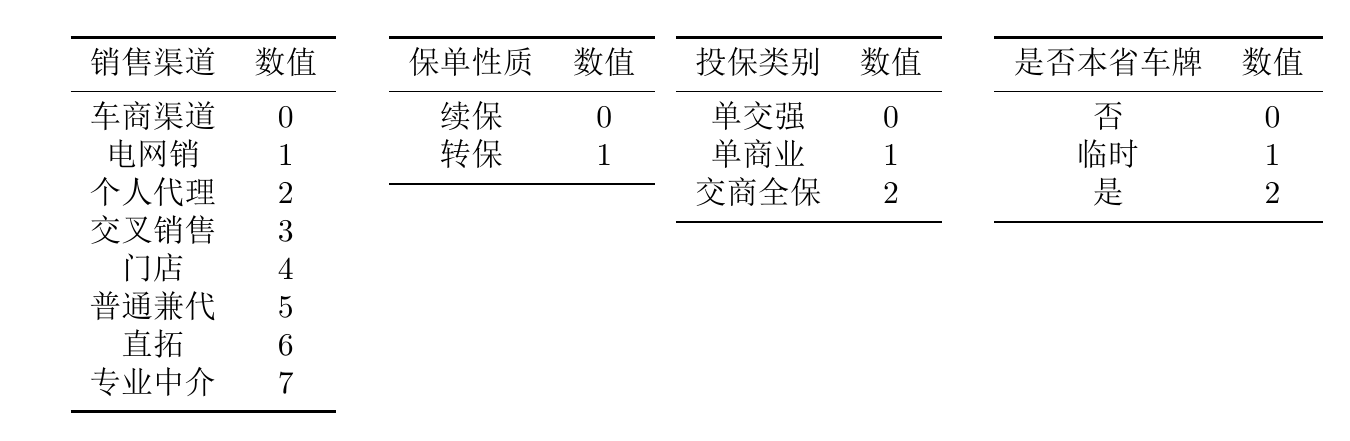
\includegraphics[scale=0.6]{transform.png}
					%\caption{}
				\end{figure}
			
				\begin{figure}[H]
					\centering
					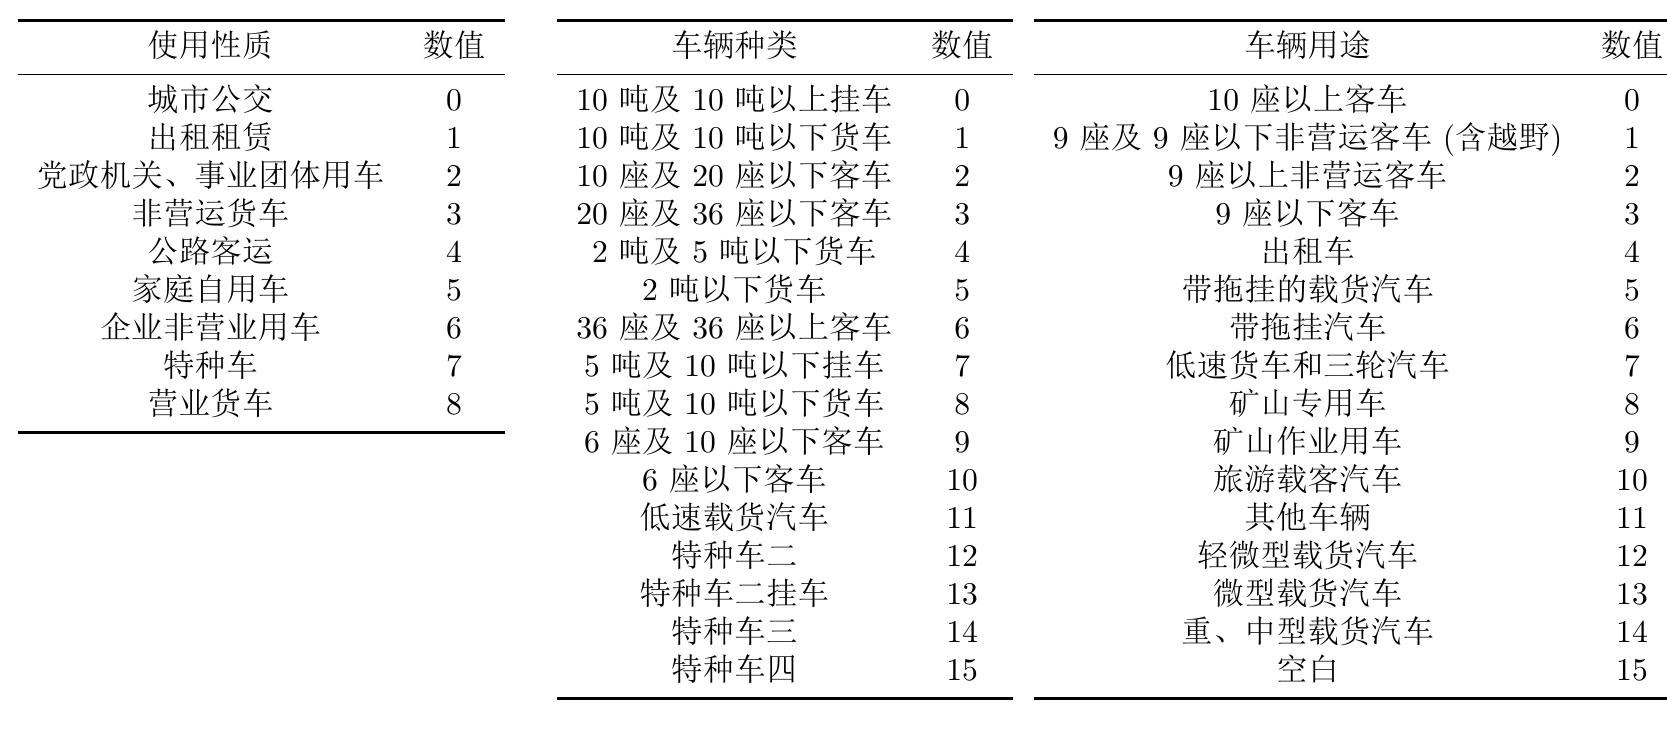
\includegraphics[scale=0.6]{transform1.png}
					\caption{属性离散化}
					\label{fig:label}
				\end{figure}
			\paragraph{}注意,上述对类别特征编码的过程中的数值n并不是指代该种类别的取值设定为n,这里我们采用的是one-hot编码规则。举例来说,对属性车辆用途来说,n = 7代表的是一个16行1列的列向量
			,其中$x_6 = 0 $,且$x_i \neq  0 $ when $i \neq  6 $。我们采用one-hot编码规则的好处是对于不能直接在属性值上计算距离的“无序属性”来说,使用one-hot编码规则能够使得使用k-mean算法得到的任意两个不同的类之间的距离都为1,从而消除距离对聚类结果的影响。有一点需要注意的是,对于某些属性来说,不同类别之间的差异不能全部简单地设置为1,因为这些类别之间的差异代表着不同的现实意义,比如,对于属性NCD的三个可能取值{连续3+无事故 连续两年无事故 上年未发生有责事故}来说,“连续3+无事故”和”连续两年无事故“所代表的驾驶能力的差别明显不同于“连续两年无事故”和“上年未发生有责事故”的驾驶能力差异。因此,对于此类的属性,我们不能简单地将其视为离散变量,而应该区分其等级。
		\subsubsection{模型建立}
			\paragraph{}首先将数据中的不同属性分别用k-mean算法进行聚类,将聚类效果明显的属性提取为我们的用户标签。当然,用户标签的提取还需要结合一定的先验知识。由于附件中属性的个数太多,这里我们只列举出聚类效果较好的几个属性,如下图所示:
					\begin{figure}[htbp]
					\centering
					\begin{minipage}[t]{0.48\textwidth}
						\centering
						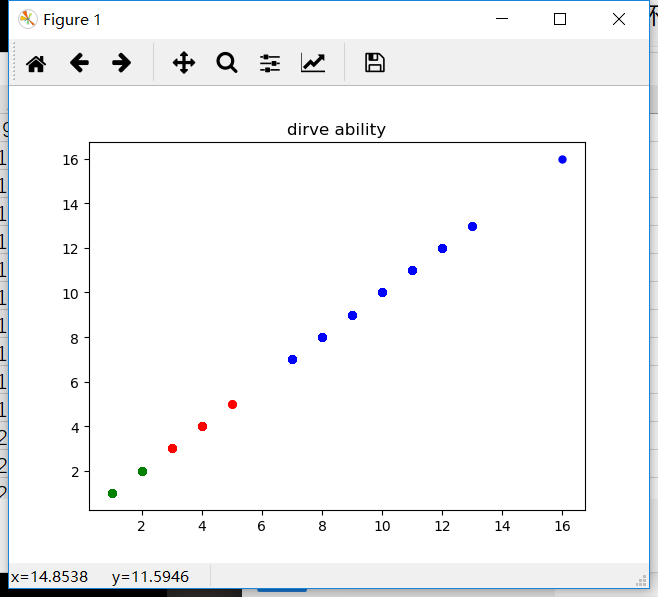
\includegraphics[scale=0.5]{cheji.png}
						\label{fig:label}
					\end{minipage}
					\begin{minipage}[t]{0.48\textwidth}
						\centering
						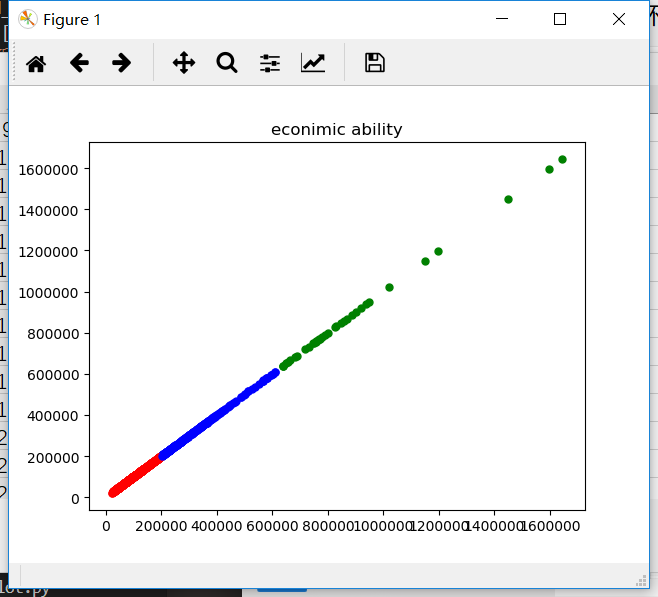
\includegraphics[scale=0.5]{jingji.png}
						\caption{经济水平聚类、驾驶习惯(技术)聚类}
					\end{minipage}
				\end{figure}
				\begin{figure}[htbp]
					\centering
					\begin{minipage}[t]{0.48\textwidth}
						\centering
						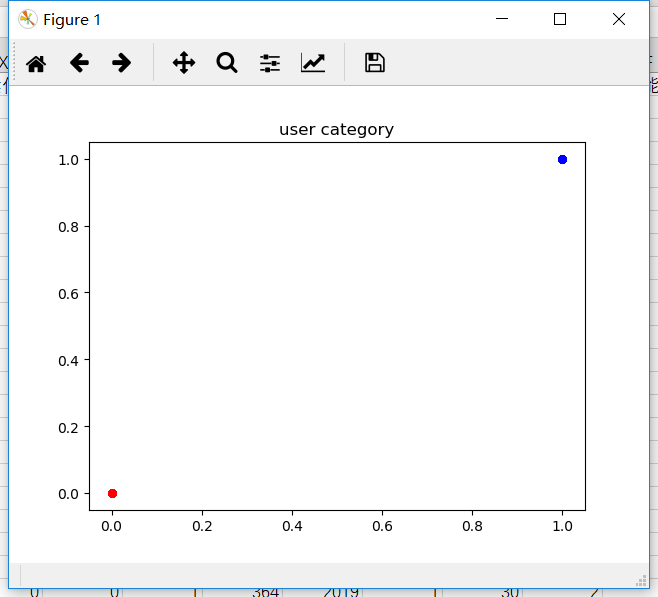
\includegraphics[scale=0.5]{2.png}
						\label{fig:label}
					\end{minipage}
					\begin{minipage}[t]{0.48\textwidth}
						\centering
						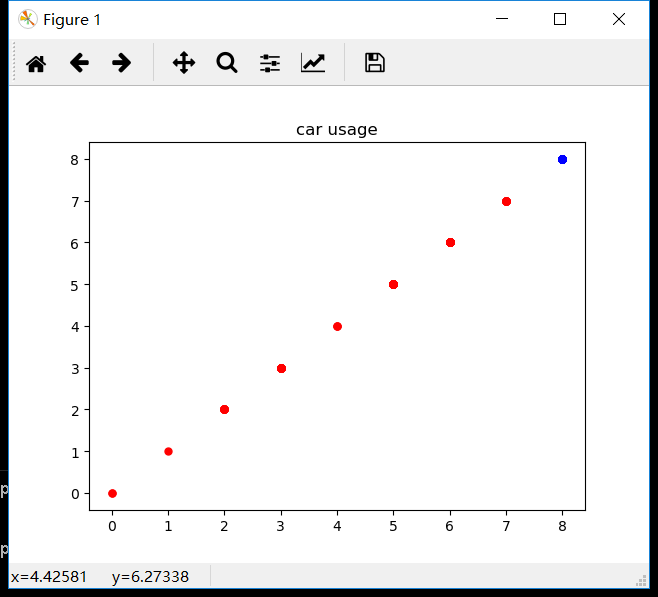
\includegraphics[scale=0.5]{car_usage.png}
						\caption{用户类别聚类与车辆用途聚类}
					\end{minipage}
				\end{figure}
			可以看到,以上几个属性的聚类效果都比较好。将以上几个属性提取为用户标签,提取的用户标签主要包括以下四个内容:\\
				\begin{figure}[H]	
					\centering
					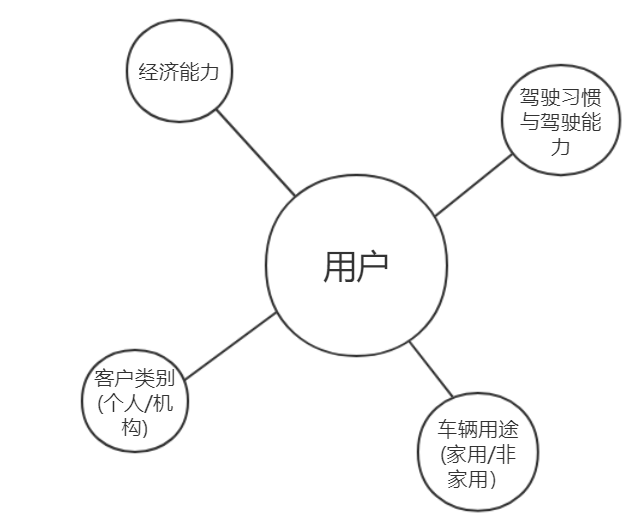
\includegraphics[scale=0.7]{model.png}
					\caption{用户画像}
				\end{figure}
			标签的取值集合为:\\
				\begin{figure}[H]	
					\centering
					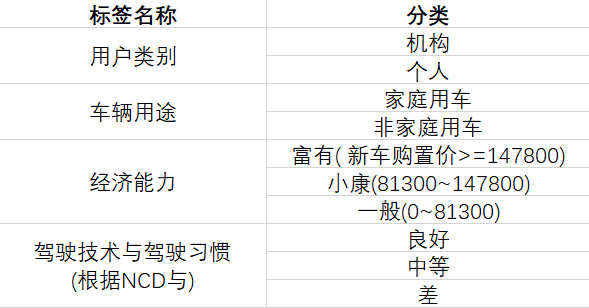
\includegraphics[scale=0.7]{1.png}
					\caption{标签的取值集合}
				\end{figure}
			确定好用户标签之后,我们将附件一的数据按照不同的类别进行分类。由于对于不同的分类类别可能适合使用不同的模型进行训练,所以将分类之后的数据分别使用逻辑回归分类器,决策树分类模型,GradientBoostingClassifier进行训练,挑选预测结果最好的模型作为该类别的学习模型。我们以模型的”准确率(precision)“和”召回率(recall)“作为预测的指标,由于根据用户标签进行分类得到的类别有很多,这里我们只给出类别A“个人用户、驾驶习惯中等、家庭用车、经济能力小康”的结果,如下所示:
				\begin{figure}[H]	
					\centering
					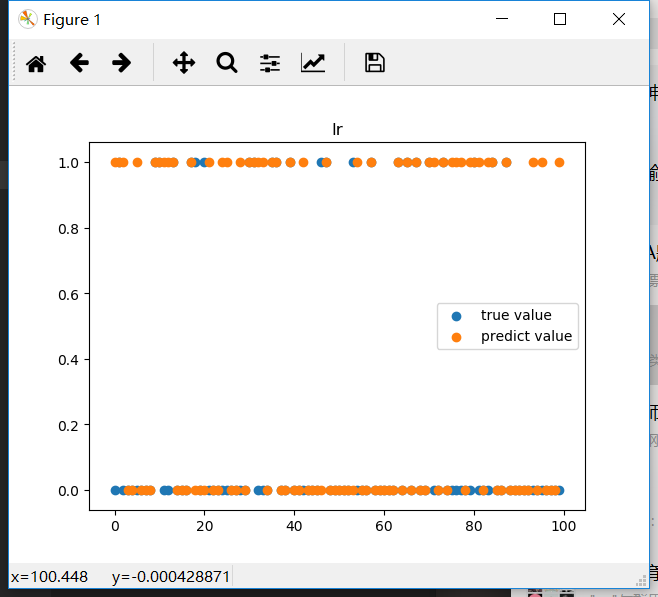
\includegraphics[scale=0.6]{lr1.png}
					\caption{logistic回归模型的预测结果}
				\end{figure}
				\begin{figure}[H]	
					\centering
					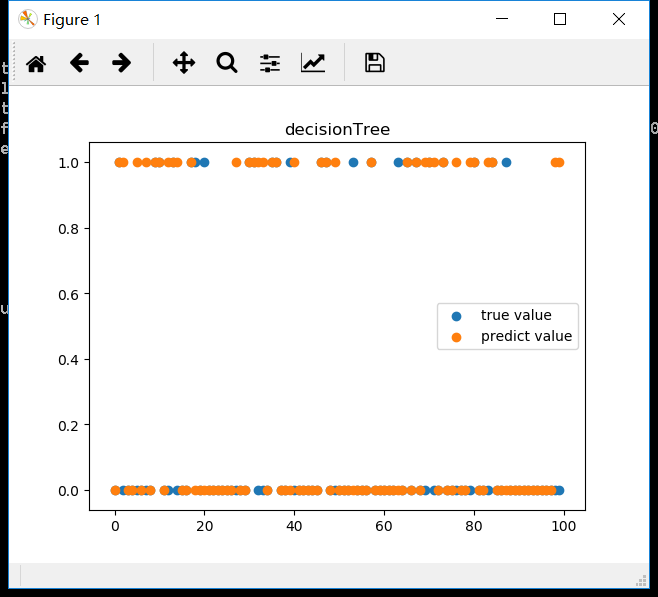
\includegraphics[scale=0.6]{lr2.png}
					\caption{l决策树模型的预测结果}
				\end{figure}
				\begin{figure}[H]	
					\centering
					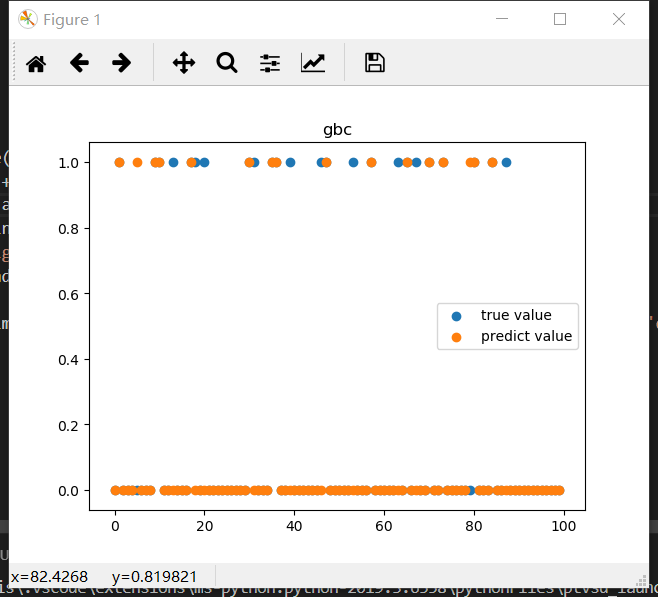
\includegraphics[scale=0.6]{gd1.png}
					\caption{GradientBoostingClassifier的预测结果}
				\end{figure}
			可以看到,对于类别A来说,logistic回归模型和决策树模型的预测效果要更好一些,具体使用哪一个模型应根据具体情况决定。
	\subsection{问题2}
		\subsubsection{问题分析}
			\paragraph{}针对不同的用户设计不同的优惠和福利方案要求我们对问题1中划分出来的所有用户类别建立各自的数学模型,模型的目标函数是最大化该类用户的续保概率。自变量为“不同的优惠和福利方案”,即保险公司可以调控的与用户相关的属性,对附件一中数据的属性进行筛选,不难发现可以用来调节以提高续保概率的因素只有“渠道”、“签单保费”、“险种”、“是否投保车损”、“是否投保车上人员”和“三者险保额”。所以“为不同的用户设计不同的优惠和福利方案”实际上要求我们调节以上属性值来尽量增大用户续保的概率。不难发现这其实是一个最优化问题,这里我们引入拉格朗日乘子法来求解这个它。
		\subsubsection{模型建立}
			\paragraph{}我们的目标函数为:
			$$ \min(1 - predict(X))$$
			约束条件为:
			$$ s.t.\begin{equation*}
			\left\{
			\begin{array}{lr}
			0 \leq x_1 \leq 1000000 &  \\
			0 \leq x_2 \\
			0 \leq x_3 \leq 7 \\
			0 \leq x_4 \leq 1 \\
			0 \leq x_5 \leq 1 \\
			0 \leq x_6 \leq 1  &
			\end{array}
			\right 
			\end{equation*} $$
			注意,这里假设$x_3,x_4,x_5,x_6$均是连续变量。
			欲提高每个用户类别的续保概率,我们只要求得每个类别对应的数学模型中目标函数的最优解即可。求解最优解可使用拉格朗日乘子法,求解最优解时的$x_1$到$x_6$的取值即确定了我们的优惠方案(假若x_1从10000变成了20000,则我们可以认为对该类别用户的优惠方案是在签单保费不变的情况下,我们可以“白送”该类顾客比原先多出的10000块险保额。其他变量的改变同理可得。),需要注意的是,若取得最优解的情况下自变量$x_1$到$x_6$中存在非整数值的应该对其取整。(属性的值不能是连续的,之前假设自变量为连续的是为便于对模型进行训练)。由于类别太多,我们只选取一个类别使用我们的模型进行分析,结果如下:
				\begin{figure}[H]	
					\centering
					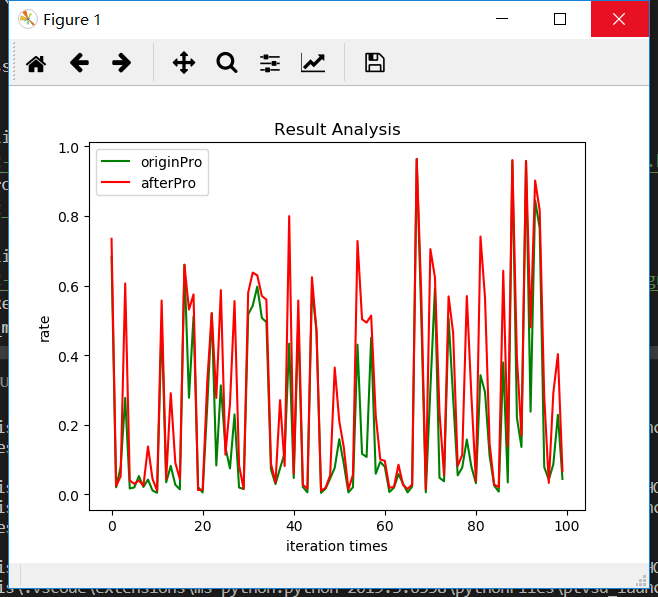
\includegraphics[scale=0.6]{result.png}
				\end{figure}
			上图中,绿色的曲线代表的是初始数据预测到的续保概率,红色曲线代表通过调节属性之后预测到的用户续保概率,从图中可以直关地看出,通过调节一些属性,我们可以做到提高用户的续保概率(推行优惠方案和福利)。
	\section{模型的验证与评价}
		\subsection{问题一}
			\paragraph{}验证我们提取的用户标签是否能够提高对客户续保概率的预测准确性,下图是直接对附件一中的数据进行建模的预测结果:
			\begin{figure}[H]	
				\centering
				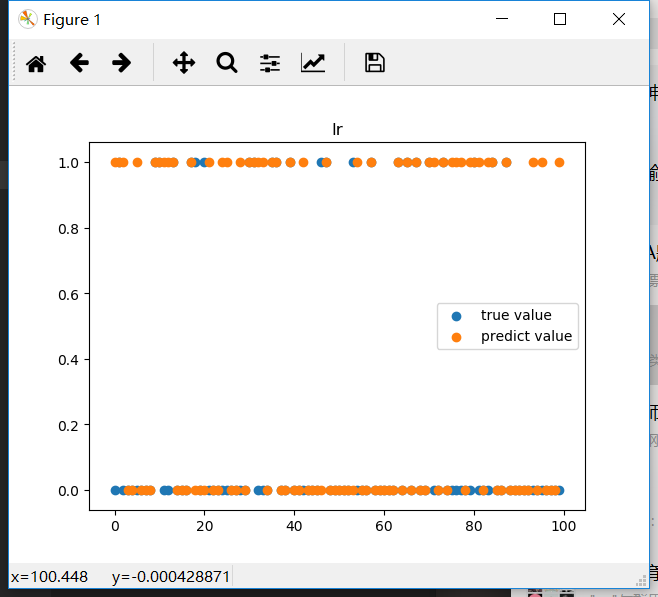
\includegraphics[scale=0.6]{lr4.png}
				\caption{logistic回归模型的预测结果}
			\end{figure}
			\begin{figure}[H]	
				\centering
				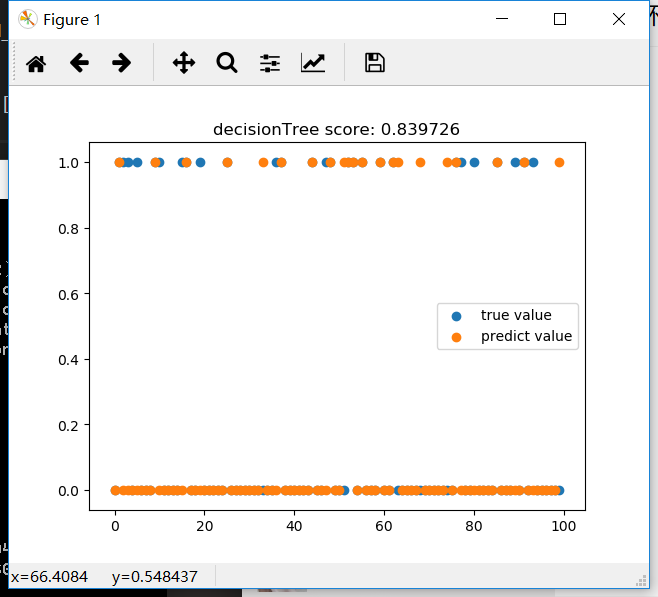
\includegraphics[scale=0.6]{dt.png}
				\caption{决策树模型的预测结果}
			\end{figure}
			\begin{figure}[H]	
				\centering
				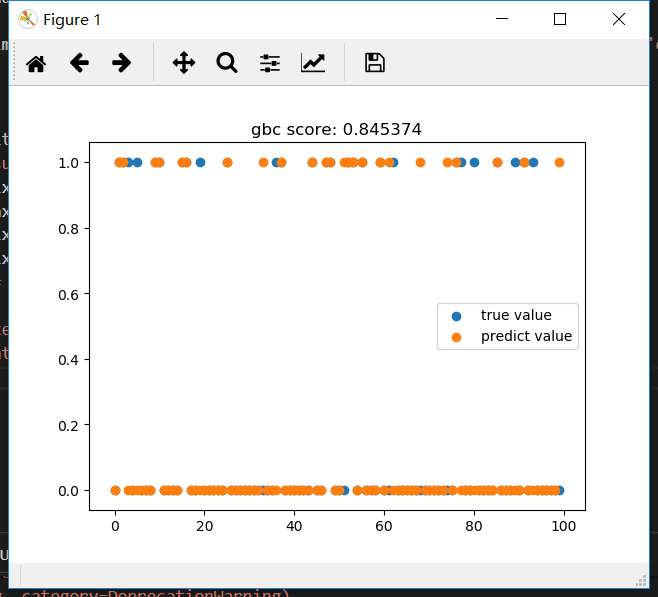
\includegraphics[scale=0.6]{gd.png}
				\caption{GradientBoostingClassifier模型的预测结果}
			\end{figure}
			我们将使用用户标签进行分类后再进行预测的结果与直接使用附件一中的所有属性进行预测的结果进行对比如下:\\ \\
			使用用户标签:
				\begin{figure}[H]	
					\centering
					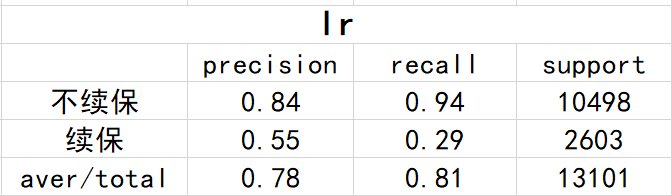
\includegraphics[scale=0.6]{lr.png}
				\end{figure}
				\begin{figure}[H]	
					\centering
					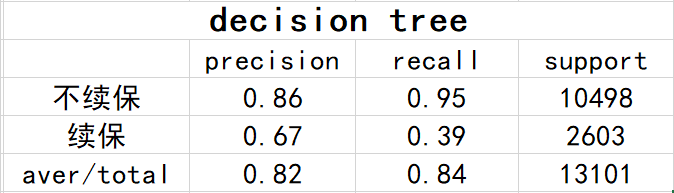
\includegraphics[scale=0.6]{decision_tree.png}
				\end{figure}
				\begin{figure}[H]	
					\centering
					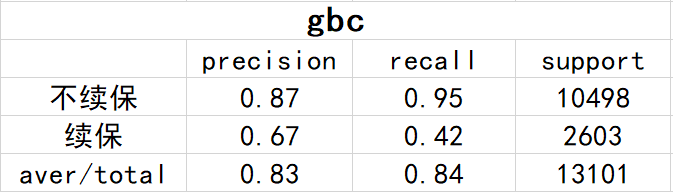
\includegraphics[scale=0.6]{gbc.png}
				\end{figure}
			初始数据:
				\begin{figure}[H]	
					\centering
					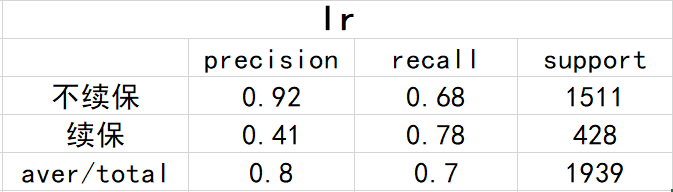
\includegraphics[scale=0.6]{lr6.png}
				\end{figure}
				\begin{figure}[H]	
					\centering
					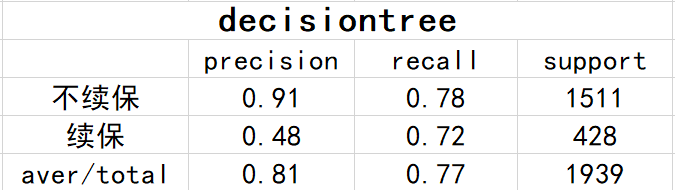
\includegraphics[scale=0.6]{decisiontree1.png}
				\end{figure}
				\begin{figure}[H]	
					\centering
					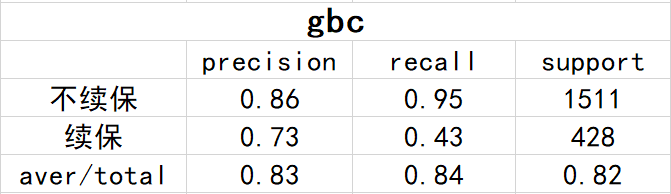
\includegraphics[scale=0.6]{gbc1.png}
				\end{figure}
		\subsection{问题二}
		\paragraph{}由于是预测模型,无法验证其结果的正确性,这里我们给出每种类别的优惠方案如下:\\
			\begin{figure}[H]	
				\centering
				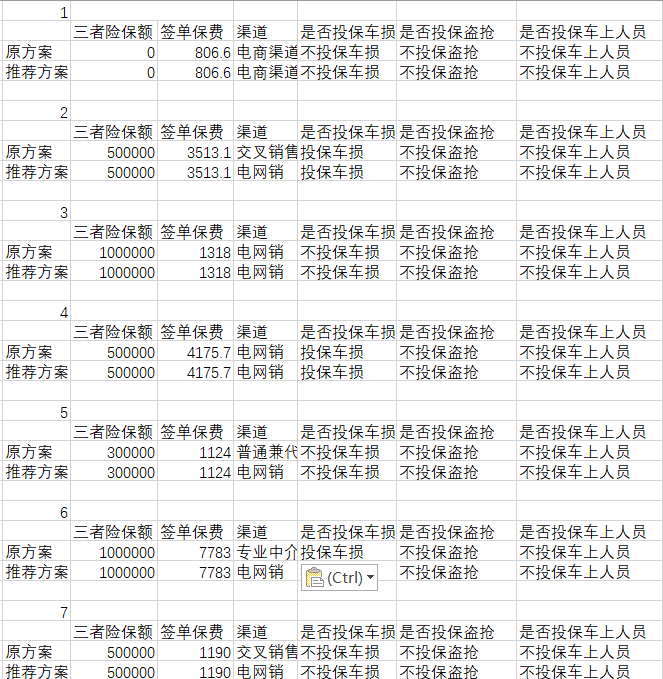
\includegraphics[scale=0.8]{111.png}
			\end{figure}
	\section{参考文献}
		\begin{thebibliography}{a}
			\bibitem{bibitem1} 作者:百度百科词条. 多元线性回归. \\
			https://baike.baidu.com/item/\%E5\%A4\%9A\%E5\%85\%83\%E7 \\
			\%BA\%BF\%E6\%80\%A7\%E5\%9B\%9E\%E5\%BD\%92/10702248?fr=aladdin.
			\bibitem{bibitem2}  周志华. 机器学习. 北京: 清华大学出版社,P403-P405 2016.
			\bibitem{bibitem3}   作者:灵夕丨月下灵 https://blog.csdn.net/xiaolong_4_2/article/details/80879337
			\bibitem{bibitem3}   作者:灵夕丨月下灵 https://blog.csdn.net/xiaolong_4_2/article/details/80879337
			\bibitem{bibitem4}   作者:人民网 http://sh.people.com.cn/n2/2017/0910/c134768-30715425.html
			
		
		\end{thebibliography}
	\section{附录}
	\paragraph{fir.py}\\
		\begin{python}
			from sklearn import preprocessing;
			import numpy as np;
			import pandas as pd;
			import matplotlib.pyplot as plt
			
			
			data = pd.read_excel("zgl.xlsx")
			
			#分类变量
			classifyVar = ['渠道', '投保类别' ,'01本省车牌', '使用性质', '车辆种类', '车辆用途',
			'险种',  '风险类别(A最低,E最高)', '客户类别', '被保险人性别', 
			'是否投保车损', '是否投保盗抢', '是否投保车上人员']
			#其余变量
			otherVar = ['NCD','车龄','被保险人年龄', '三者险保额',  '新车购置价', '签单保费','立案件数', '已决赔款']
			
			X = data.iloc[:, 0:37]
			Y = data.iloc[:, 37]
			print(Y)
			#data = data.drop(columns=[])
			
			Xclassify = X[classifyVar]
			
			Xother = X[otherVar]
			
			
			#进行数据预处理,对分类变量和普通变量分别进行One-hot编码以及归一化
			from sklearn import preprocessing
			ss_x = preprocessing.StandardScaler()
			oneH_enc = preprocessing.OneHotEncoder()
			Xother = ss_x.fit_transform(Xother)
			Xclassify = oneH_enc.fit_transform(Xclassify)
			
			from scipy.sparse import hstack
			X = hstack((Xother, Xclassify))
			
			#划分训练集和验证集
			from sklearn.cross_validation import train_test_split,cross_val_score
			X_train, X_test, Y_train, Y_test = train_test_split(X, Y, test_size=0.2,  random_state=4)
			
			from sklearn.metrics import classification_report
			def try_different_method(model, name):
			model.fit(X_train,Y_train)
			#scores = cross_val_score(model,X_train,Y_train,cv=5).ravel()
			#score = np.mean(scores)
			print (model.predict_proba(X_test))
			'''score = model.score(X_test, Y_test)'''
			result = model.predict(X_test)
			
			plt.figure()
			plt.scatter(np.arange(100),  Y_test[:100],  label='true value')
			plt.scatter(np.arange(100), result[:100],  label='predict value')
			#plt.title(name + ' score: %f'%score)
			plt.legend()
			plt.show()
			
			print(classification_report(Y_test, result, target_names=['不续保', '续保']))
			
			
			from sklearn.linear_model import Perceptron
			#http://scikit-learn.org/stable/modules/generated/sklearn.linear_model.Perceptron.html#sklearn.linear_model.Perceptron
			ppn = Perceptron()
			#try_different_method(ppn, 'perceptron')
			
			from sklearn.linear_model import LogisticRegression
			#http://scikit-learn.org/stable/modules/generated/sklearn.linear_model.LogisticRegression.html#sklearn.linear_model.LogisticRegression
			lr = LogisticRegression(C=1000.0, random_state=0)
			try_different_method(lr, 'lr')
			
			
			from sklearn.svm import SVC
			#http://scikit-learn.org/stable/modules/generated/sklearn.svm.SVC.html#sklearn.svm.SVC
			svm = SVC(kernel='linear', C=1.0, random_state=0,probability=True)
			#try_different_method(svm, 'svc')
			
			from sklearn.tree import DecisionTreeClassifier
			#http://scikit-learn.org/stable/modules/generated/sklearn.tree.DecisionTreeClassifier.html#sklearn.tree.DecisionTreeClassifier
			tree = DecisionTreeClassifier(criterion='entropy', max_depth=10, random_state=0)
			try_different_method(tree, 'decisionTree')
			
			from sklearn.ensemble import RandomForestClassifier
			forest = RandomForestClassifier(criterion='entropy', n_estimators=10, random_state=1, n_jobs=2)
			#http://scikit-learn.org/stable/modules/generated/sklearn.ensemble.RandomForestClassifier.html#sklearn.ensemble.RandomForestClassifier
			#criterion特征选择度量,n_estimators随机森林中单棵树数目,n_jobs设置并行生成树模型得数目
			try_different_method(forest, 'RandomForest')
			
			from sklearn.tree import ExtraTreeClassifier 
			ExtraTree = ExtraTreeClassifier()
			try_different_method(ExtraTree, 'ExtraTree')
			
			from sklearn.ensemble import BaggingClassifier
			Bagging = BaggingClassifier()
			try_different_method(Bagging, 'Bagging')
			
			from sklearn.ensemble import GradientBoostingClassifier
			gbc = GradientBoostingClassifier()
			try_different_method(gbc, 'gbc')
		\end{python}
		\paragraph{sec.py}\\
		\begin{*sec.py*}
			from sklearn import preprocessing;
			import numpy as np;
			import pandas as pd;
			import matplotlib.pyplot as plt
			
			
			data = pd.read_excel("C:\\Users\\artemis\\Desktop\\认证杯\\test\\data2\\3.xlsx")
			
			
			#分类变量
			classifyVar = ['投保类别' ,'01本省车牌', '使用性质', '车辆种类', '车辆用途',
			'险种',  '风险类别(A最低,E最高)', '客户类别', '被保险人性别', 
			'渠道', '是否投保车损', '是否投保盗抢', '是否投保车上人员']
			#其余变量
			otherVar = ['NCD','车龄','被保险人年龄', '新车购置价', '立案件数', '已决赔款', '三者险保额', '签单保费' ]
			
			X = data.iloc[:, 0:]
			Y = data.iloc[:, 36]
			#print(Y)
			#data = data.drop(columns=[])
			
			Xclassify = X[classifyVar]
			
			Xother = X[otherVar]
			
			
			#进行数据预处理,对分类变量和普通变量分别进行One-hot编码以及归一化
			from sklearn import preprocessing
			ss_x = preprocessing.StandardScaler()
			oneH_enc = preprocessing.OneHotEncoder()
			Xother = ss_x.fit_transform(Xother)
			Xclassify = oneH_enc.fit_transform(Xclassify)
			
			from scipy.sparse import hstack
			X = hstack((Xother, Xclassify))
			
			#划分训练集和验证集
			from sklearn.cross_validation import train_test_split,cross_val_score
			X_train, X_test, Y_train, Y_test = train_test_split(X, Y, test_size=0.2,  random_state=4)
			
			from sklearn.metrics import classification_report
			def try_different_method(model, name):
			model.fit(X_train,Y_train)
			#scores = cross_val_score(model,X_train,Y_train,cv=5).ravel()
			#score = np.mean(scores)
			print (model.predict_proba(X_test))
			'''score = model.score(X_test, Y_test)'''
			result = model.predict(X_test)
			
			plt.figure()
			plt.scatter(np.arange(100),  Y_test[:100],  label='true value')
			plt.scatter(np.arange(100), result[:100],  label='predict value')
			plt.title(name)
			plt.legend()
			plt.show()
			
			print(classification_report(Y_test, result, target_names=['不续保', '续保']))
			
			
			from sklearn.linear_model import Perceptron
			#http://scikit-learn.org/stable/modules/generated/sklearn.linear_model.Perceptron.html#sklearn.linear_model.Perceptron
			ppn = Perceptron()
			#try_different_method(ppn, 'perceptron')
			
			from sklearn.linear_model import LogisticRegression
			#http://scikit-learn.org/stable/modules/generated/sklearn.linear_model.LogisticRegression.html#sklearn.linear_model.LogisticRegression
			lr = LogisticRegression(C=1000.0, random_state=0, class_weight='balanced')
			try_different_method(lr, 'lr', )
			
			
			from sklearn.svm import SVC
			#http://scikit-learn.org/stable/modules/generated/sklearn.svm.SVC.html#sklearn.svm.SVC
			svm = SVC(kernel='linear', C=1.0, random_state=0,probability=True)
			#try_different_method(svm, 'svc')
			
			from sklearn.tree import DecisionTreeClassifier
			#http://scikit-learn.org/stable/modules/generated/sklearn.tree.DecisionTreeClassifier.html#sklearn.tree.DecisionTreeClassifier
			tree = DecisionTreeClassifier(criterion='entropy', max_depth=10, random_state=0, class_weight='balanced')
			try_different_method(tree, 'decisionTree')
			
			from sklearn.ensemble import RandomForestClassifier
			forest = RandomForestClassifier(criterion='entropy', n_estimators=10, random_state=1, n_jobs=2, class_weight='balanced')
			#http://scikit-learn.org/stable/modules/generated/sklearn.ensemble.RandomForestClassifier.html#sklearn.ensemble.RandomForestClassifier
			#criterion特征选择度量,n_estimators随机森林中单棵树数目,n_jobs设置并行生成树模型得数目
			#try_different_method(forest, 'RandomForest')
			
			from sklearn.tree import ExtraTreeClassifier 
			ExtraTree = ExtraTreeClassifier(class_weight='balanced')
			try_different_method(ExtraTree, 'ExtraTree')
			
			from sklearn.ensemble import BaggingClassifier
			Bagging = BaggingClassifier()
			#try_different_method(Bagging, 'Bagging')
			
			from sklearn.ensemble import GradientBoostingClassifier
			gbc = GradientBoostingClassifier()
			try_different_method(gbc, 'gbc')
			
			'''第二问'''
			
			#目标样本
			index = 0
			
			
			secondData =pd.read_excel("C:\\Users\\artemis\\Desktop\\认证杯\\test\\data2\\3.xlsx")
			
			secondX = secondData.iloc[:, 0:]
			
			
			secClassifyVar = ['投保类别' ,'01本省车牌', '使用性质', '车辆种类', '车辆用途',
			'险种', '风险类别(A最低,E最高)', '客户类别', '被保险人性别']
			secOtherVar = ['NCD', '车龄', '被保险人年龄', '新车购置价',  '立案件数', '已决赔款']
			
			targetVar = [ '三者险保额' , '签单保费', '渠道', '是否投保车损', '是否投保盗抢', '是否投保车上人员']
			
			
			origin = secondX[targetVar].values
			
			
			#进行数据预处理,对分类变量和普通变量分别进行One-hot编码以及归一化
			# from sklearn import preprocessing
			# ss_x = preprocessing.StandardScaler()
			# oneH_enc = preprocessing.OneHotEncoder()
			# Xother = ss_x.fit_transform(Xother)
			# Xclassify = oneH_enc.fit_transform(Xclassify)
			
			
			#预测模型,可以进行调整
			model = gbc
			
			delta = 0.0001
			
			from scipy.optimize import minimize
			#优化的目标函数
			def func(args):
			""" 定义目标函数F(x) """
			
			args = np.array(args)
			Xclassify = secondX[secClassifyVar].values[index].tolist()
			Xclassify.append(args[2])
			Xclassify.append(args[3])
			Xclassify.append(args[4])
			Xclassify.append(args[5])
			
			Xother = secondX[secOtherVar].values[index].tolist()
			Xother.append(args[0])
			Xother.append(args[1])
			
			Xother = np.array(Xother)
			Xclassify = np.array(Xclassify)
			
			Xother = Xother.reshape(-1,1).transpose()
			Xclassify = Xclassify.reshape(-1,1).transpose()
			
			
			Xother = ss_x.transform(Xother)
			Xclassify = oneH_enc.transform(Xclassify)
			
			from scipy.sparse import hstack
			testX = hstack((Xother, Xclassify))
			
			#print(testX)
			
			prob = model.predict_proba(testX)
			#print(prob)
			result = prob[0][0]
			return result * 10000
			
			cons = ({'type': 'ineq',#不等式约束条件
				'fun' : lambda x: x[0] - delta},
			{'type': 'ineq',#不等式约束条件
				'fun' : lambda x: 2000000 - x[0] - delta},
			{'type': 'ineq',#不等式约束条件
				'fun' : lambda x: x[1] - delta},
			{'type': 'ineq',#不等式约束条件
				'fun' : lambda x: 1 - x[2] - delta},
			{'type': 'ineq',#不等式约束条件
				'fun' : lambda x: x[2] - delta},
			{'type': 'ineq',#不等式约束条件
				'fun' : lambda x: 1 - x[3] - delta},
			{'type': 'ineq',#不等式约束条件
				'fun' : lambda x: x[3] - delta},
			{'type': 'ineq',#不等式约束条件
				'fun' : lambda x: 1 - x[4] - delta},
			{'type': 'ineq',#不等式约束条件
				'fun' : lambda x: x[4] - delta},
			{'type': 'ineq',#不等式约束条件
				'fun' : lambda x: 1 - x[5] - delta},
			{'type': 'ineq',#不等式约束条件
				'fun' : lambda x: x[5] - delta},
			)
			
			#初值
			
			
			originPro = []
			afterPro = []
			for i in range(100):
			index = i + 5000
			originPro.append(model.predict_proba(X.toarray()[index].reshape(-1,1).transpose())[0][1])
			print(X.toarray()[index].reshape(-1,1).transpose())
			x0 = origin[index]
			#print('originalChioce: ')
			#print(Y[index])
			#print(x0)
			print('original plan')
			print(x0)
			res = minimize(func, x0, args=(), constraints=cons, method='SLSQP', options={'disp': True})
			afterPro.append(1- res.fun / 10000)
			print('new plan')
			print(res.x)
			
			#开始画图
			plt.title('Result Analysis')
			plt.plot(range(100), originPro, color='green', label='originPro')
			plt.plot(range(100), afterPro, color='red', label='afterPro')
			plt.legend() # 显示图例
			
			plt.xlabel('iteration times')
			plt.ylabel('rate')
			plt.show()
		\end{*sec.py*}
		\paragraph{user.py}\\
		\begin{1}
			import numpy as np;
			import pandas as pd;
			import matplotlib.pyplot as plt
			
			targetFactor = '新老用户'
			data = pd.read_excel("real2(2).xlsx")
			originalVar = ['保单性质']
			otherVar = ['续保年']
			
			
			X = data.iloc[:, 2:26]
			Xoriginal = X[originalVar]
			Xother = X[otherVar]
			
			#进行数据预处理,对分类变量和普通变量分别进行One-hot编码以及归一化
			from sklearn import preprocessing
			ss_x = preprocessing.StandardScaler()
			Xother = ss_x.fit_transform(Xother)
			oneH_enc = preprocessing.OneHotEncoder()
			Xoriginal = oneH_enc.fit_transform(Xoriginal)
			
			from scipy.sparse import hstack
			X_train = hstack((Xoriginal, Xother))
			
			from sklearn.cluster import KMeans
			#分类个数
			n_clusters = 2
			kmean = KMeans(n_clusters=n_clusters)
			kmean.fit(X_train)
			print(kmean.labels_)
			
			
			
			
			originalVar.extend(otherVar)
			data_list = X[originalVar].values
			originalVar.append(targetFactor)
			
			labels = kmean.labels_[:, np.newaxis]
			data_list = np.hstack((data_list, labels))
			
			
			strat_df1 = pd.DataFrame(data=data_list, columns=originalVar)
			
			writer = pd.ExcelWriter((targetFactor + '.xlsx'))
			strat_df1.to_excel(writer, 'Sheet1')
			writer.save()
		\end{1}
	
	
	
\end{document} 